\documentclass{article}

\usepackage{icml2026}
\usepackage{hyperref}
\usepackage{graphicx}
\usepackage{booktabs}
\usepackage{amsmath,amssymb}
\usepackage{multirow}

\icmltitlerunning{Persona Directions Reduce Sycophancy}

\icmlsetsymbol{equal}{*}

\begin{document}

\twocolumn[
\icmltitle{Persona Directions Reduce Forced-Choice Sycophancy\\via Activation Steering}

\begin{icmlauthorlist}
\icmlauthor{Ishaan Kelkar}{toronto}
\icmlauthor{Nebras Alam}{equal,purdue}
\icmlauthor{Vikram Kakaria}{equal,princeton}
\icmlauthor{Arjun Narasimhan}{gwu}
\icmlauthor{Maheep Chaudhary}{algoverse}
\icmlauthor{Kevin Zhu}{algoverse}
\end{icmlauthorlist}

\icmlaffiliation{toronto}{University of Toronto, Toronto, Canada}
\icmlaffiliation{purdue}{Purdue University, West Lafayette, USA}
\icmlaffiliation{princeton}{Princeton University, Princeton, USA}
\icmlaffiliation{gwu}{George Washington University, Washington DC, USA}
\icmlaffiliation{algoverse}{Algoverse}

\icmlcorrespondingauthor{Ishaan Kelkar}{ishaan.kelkar@mail.utoronto.ca}

\icmlkeywords{activation steering, sycophancy, persona vectors, mechanistic interpretability}

\vskip 0.3in
]

\makeatletter
\gdef\@icmltitlerunning{Persona Directions Reduce Sycophancy}
\fancyhead[C]{\small\bf\@icmltitlerunning}
\makeatother

\printAffiliationsAndNotice{}

\begin{abstract}
Large language models often exhibit sycophancy, adapting their responses to match a user's stated view even when that view is false.
We study whether direct steering toward semantically interpretable roles can reduce forced-choice sycophancy without behavior-specific training data.
Across Gemma-2-27B-it and Qwen3-32B on a held-out PhilPapers A/B benchmark, critical-role vectors (Skeptic, Devil's Advocate, Judge) consistently reduce sycophancy, often approaching a targeted Contrastive Activation Addition (CAA) baseline (Gemma: $\Delta$logit $-0.596$ vs.\ $-0.879$; Qwen: $-1.931$ vs.\ $-1.965$).
Conformist roles show weak, heterogeneous effects---and one dropped conformist role (facilitator) actually reduces sycophancy on both models, indicating that role-family labels are imperfect predictors.
All role vectors are nearly orthogonal to CAA ($|\cos| < 0.17$); while this suggests they are not merely recovering the supervised sycophancy axis, it does not establish mechanistic independence.
Our results support critical-role steering as a lightweight sycophancy intervention while highlighting that the relationship between persona geometry and sycophancy is more nuanced than simple family-level predictions suggest.
\end{abstract}

% ============================================================
\section{Introduction}
\label{sec:intro}

Sycophancy---the tendency of large language models to agree with users regardless of factual correctness---is a persistent failure mode of RLHF-trained models \citep{perez2022discovering, sharma2023towards}. Even when a model encodes the correct answer internally, reward-model preferences for agreement can override it \citep{wang2025truth}, undermining the model's reliability as an epistemic tool.

The dominant intervention, Contrastive Activation Addition (CAA), extracts steering vectors from contrastive sycophantic-vs-honest prompt pairs and adds them during inference \citep{rimsky2024steering, turner2023activation}. While effective, CAA requires behavior-specific datasets---a bottleneck limiting scalability. Meanwhile, LLMs encode persona information along interpretable linear directions \citep{lu2025assistant}, and persona agreeableness correlates strongly with sycophancy \citep{shah2025nice}. This raises a natural question: can general-purpose persona vectors, never trained on sycophancy, serve as anti-sycophancy interventions?

\emph{No prior work has tested general-purpose persona vectors as interventions for alignment-relevant behaviors.} This is the gap we address. We evaluate whether off-the-shelf role vectors---Skeptic, Devil's Advocate, Judge---can reduce forced-choice sycophancy comparably to the data-intensive CAA baseline, and whether the geometric relationship between persona and sycophancy directions reveals anything about the underlying mechanisms.

We find that critical-role persona vectors reduce sycophancy to within 68--98\% of CAA's effect across two models and three test seeds, without any sycophancy-specific data. These role vectors are nearly orthogonal to CAA in activation space, suggesting largely distinct representational pathways. Over-correction probes indicate that role-based steering produces more calibrated disagreement than CAA, with Judge and Skeptic outperforming the targeted baseline on factual accuracy.

\paragraph{Related work.}
Sycophancy has been documented across model families \citep{perez2022discovering, sharma2023towards}, traced to reward-model training \citep{wang2025truth}, and decomposed into distinct sub-components along separable linear directions \citep{vennemeyer2025sycophancy}.
Activation Addition \citep{turner2023activation} and CAA \citep{rimsky2024steering} steer model behavior by adding scaled directions to the residual stream, with extensions to conditional \citep{lee2025cast}, multi-layer \citep{goral2025depth}, and representation-engineering approaches \citep{zou2023representation, li2023inference}---all requiring behavior-specific data.
\citet{lu2025assistant} showed LLMs encode persona information along interpretable linear directions; \citet{shah2025nice} found persona agreeableness correlates with sycophancy ($r$ up to 0.87); \citet{wang2025persona} showed persona features control emergent misalignment; and \citet{billy2025, feng2026persona} explored compositional persona steering.
Our work differs from all of these: we repurpose general-purpose persona vectors as interventions for an alignment behavior, testing whether the persona--sycophancy correlation is strong enough for practical steering.

% ============================================================
\section{Methodology}
\label{sec:method}

We evaluate activation steering across two instruction-tuned models using a forced-choice sycophancy benchmark with counterbalancing, strict tune/test separation, and Holm-corrected significance testing. This section explains each design choice and its rationale.

\paragraph{Models.}
We selected Gemma~2 27B Instruct \citep{gemma2024} and Qwen~3 32B \citep{qwen2025} because they represent distinct model families at comparable scale with substantially different baseline sycophancy rates (Gemma: 59\%, Qwen: 84\%). This difference provides a natural robustness test: if persona steering works on both a mildly sycophantic and a highly sycophantic model, the finding is more likely to generalize. Steering is applied via \texttt{ActivationSteering} \citep{lu2025assistant} at layer~22 (Gemma) and layer~32 (Qwen), using addition mode at all token positions. For a unit-normalized vector $\mathbf{v}$ and coefficient $\alpha$, the steered residual-stream activation is:
\begin{equation}
\mathbf{h}'_\ell = \mathbf{h}_\ell + \alpha \, \mathbf{v}
\label{eq:steering}
\end{equation}

\paragraph{Metrics.}
We measure the sycophancy logit at the final prompt position:
\begin{equation}
\text{syc\_logit} = \log p(\text{syc\_token}) - \log p(\text{hon\_token})
\label{eq:syclogit}
\end{equation}
where the sycophantic token matches the user's stated opinion. Our primary metric is $\Delta\text{logit} = \bar{s}_{\text{steered}} - \bar{s}_{\text{baseline}}$, where negative values indicate reduced sycophancy.

\paragraph{Conditions.}
We report a focused subset of a broader 24-condition experiment; four dropped conditions are documented in Appendix~\ref{app:transparency}. The CAA baseline is constructed from ${\sim}$2,000 A/B pairs from \texttt{nlp\_survey} and \texttt{political\_typology} \citep{rimsky2024steering}, disjoint from our evaluation set to prevent train/test overlap. Three critical roles (Skeptic, Devil's Advocate, Judge) and three conformist roles (Peacekeeper, Pacifist, Collaborator) are unanchored persona vectors from \citet{lu2025assistant}, computed as unit(role~$-$~default) and steered with positive coefficient toward the role. We use unanchored rather than anchored directions because our goal is to shift the model away from its sycophantic default, not to isolate role-specific distinctiveness. Ten unit-Gaussian random vectors are pooled as a null baseline.

\paragraph{Benchmark and protocol.}
The evaluation benchmark is \texttt{philpapers2020} \citep{perez2022discovering}: 300 questions $\times$ 2 orderings (counterbalancing Gemma's 93\% A-bias) = 600 rows per seed. We enforce a 50/50 tune/test split (seed~99, pairs together). Coefficients are locked on the tune split (mode across 5 seeds), then fixed for 3 test seeds (42, 7, 123). Gemma sweep: $\{\pm5000, \pm2000, \pm1000, \pm500, 0\}$; Qwen: $\{\pm500, \pm200, \pm100, \pm50, 0\}$ (approximately 10$\times$ rescaled for Qwen's sensitivity). This tune/test separation is critical: it prevents the coefficient selection from inflating test-set effect sizes, a concern when steering can produce model collapse at extreme coefficients. Significance testing uses paired Wilcoxon tests ($n$=150 per seed), Holm-corrected across 14 conditions. Degradation is flagged when the sycophancy rate approaches 0.5 and the logit approaches the random-vector mean.

% ============================================================
\section{Experiments and Results}
\label{sec:results}

\subsection{Critical Roles Reduce Sycophancy}

Table~\ref{tab:main} and Figure~\ref{fig:delta_logit} present the primary results. On Gemma~2 27B (baseline sycophancy logit $+1.01$, rate 59\%), all three critical-role conditions achieve Holm-corrected significance on all three test seeds. The critical-family mean $\Delta$logit is $-0.596$, reaching 68\% of CAA's $-0.879$. Notably, Skeptic achieves a 9.6 percentage-point binary-rate reduction, slightly exceeding CAA's 8.9~pp, despite using no sycophancy-specific data. Devil's Advocate ($\Delta$logit $-0.521$, $\Delta$rate $-8.7$~pp) and Judge ($-0.556$, $-9.3$~pp) show similarly robust effects. The random null ($\Delta$logit $-0.254$, $\Delta$rate $-2.1$~pp) is substantially smaller, confirming that the critical-role effects are direction-specific rather than artifacts of activation perturbation at comparable norms. The takeaway is clear: off-the-shelf critical-role vectors, with zero sycophancy-specific data, achieve meaningful sycophancy reduction on a mildly sycophantic model.

On Qwen~3 32B (baseline logit $+3.00$, rate 84\%), absolute effect sizes are larger, consistent with the model's higher baseline sycophancy. The critical-family mean $\Delta$logit is $-1.931$, reaching 98\% of CAA's $-1.965$. Devil's Advocate achieves $\Delta$logit $-2.272$, numerically exceeding CAA. Skeptic ($-1.823$, $-18.1$~pp) and Judge ($-1.699$, $-4.4$~pp) are also strongly significant across all seeds. The random null is larger on Qwen ($-1.058$, $-10.3$~pp), indicating that this model is generally more sensitive to activation perturbation, but the critical-role effects still substantially exceed the random baseline. Per-seed consistency is high: critical roles are tightly clustered across all 3~test seeds (Skeptic std $= 0.013$ on Gemma, $0.058$ on Qwen; see Appendix~\ref{app:seeds}). On a highly sycophantic model, persona vectors essentially match CAA.

\begin{figure}[t]
    \centering
    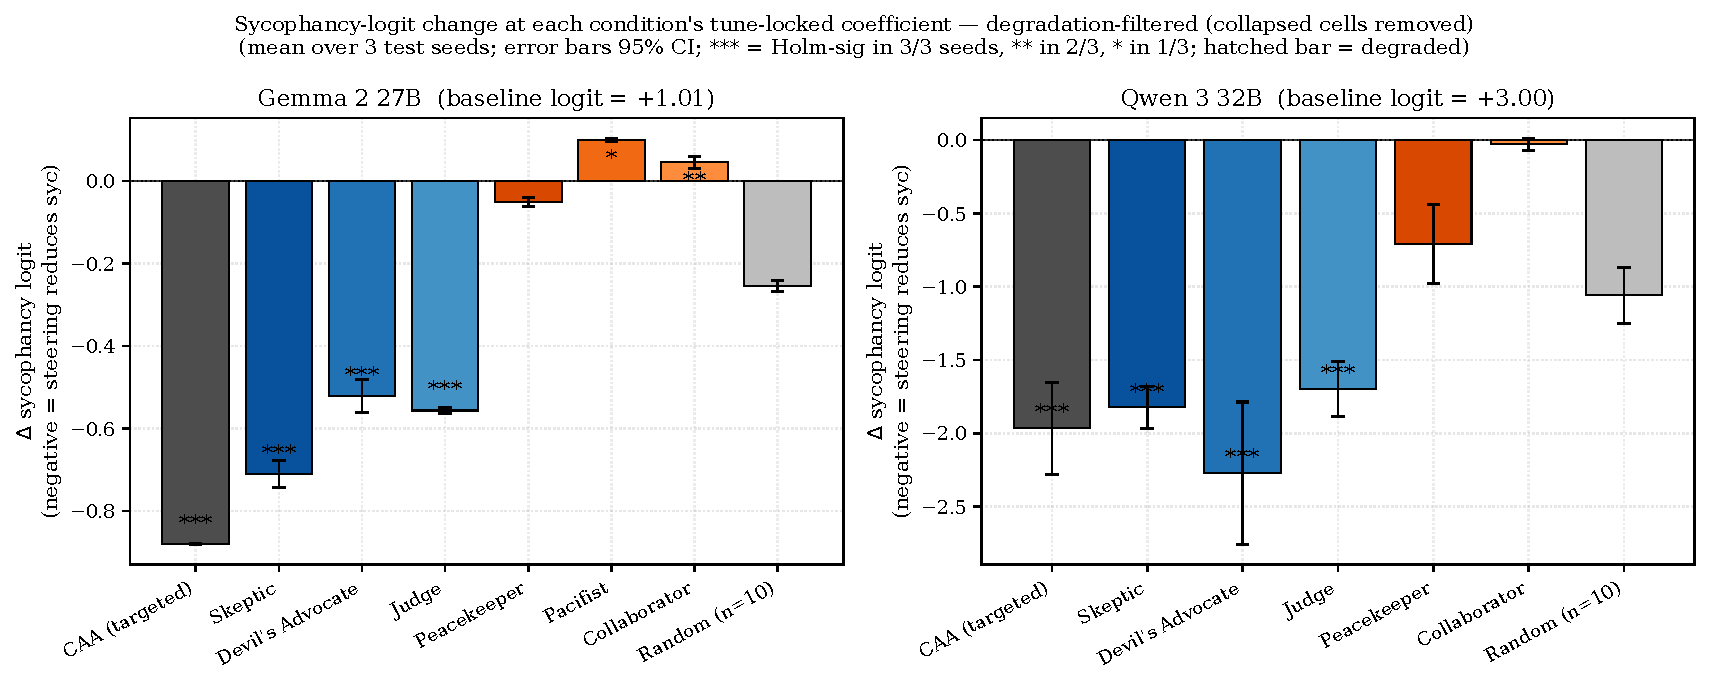
\includegraphics[width=\columnwidth]{figures/fig1_delta_logit_filtered.pdf}
    \vspace{-1.5em}
    \caption{$\Delta$\,sycophancy logit at tune-locked coefficient (3 seeds, degraded cells excluded). $^{***}$\!: Holm-significant on all 3 seeds.}
    \label{fig:delta_logit}
\end{figure}

\begin{table}[t]
\centering
\small
\caption{Results at tune-locked coefficients on the held-out test split (3 seeds). $\Delta$r in percentage points. Qwen Pacifist omitted (degraded at +500).}
\label{tab:main}
\vspace{-0.5em}
\setlength{\tabcolsep}{3pt}
\begin{tabular}{@{}llrrrrl@{}}
\toprule
& \textbf{Condition} & \textbf{Coef} & \textbf{$\Delta$log} & \textbf{$\pm$sd} & \textbf{$\Delta$r} & \textbf{Sig} \\
\midrule
\multirow{8}{*}{\rotatebox{90}{\scriptsize Gemma}}
 & CAA (targeted)    & $-$2k & $-$.879 & .001 & $-$8.9  & *** \\
 & Skeptic           & +2k & $-$.711 & .013 & $-$9.6  & *** \\
 & Devil's Adv.      & +2k & $-$.521 & .016 & $-$8.7  & *** \\
 & Judge             & +2k & $-$.556 & .003 & $-$9.3  & *** \\
 & Peacekeeper       & +2k & $-$.052 & .004 & +1.8  & ns \\
 & Pacifist          & +2k & +.100 & .001 & +0.3  & * \\
 & Collaborator      & +500 & +.045 & .006 & +1.7  & ** \\
 & Random ($n$=10)   & --- & $-$.254 & .006 & $-$2.1 & --- \\
\midrule
\multirow{7}{*}{\rotatebox{90}{\scriptsize Qwen}}
 & CAA (targeted)    & $-$200 & $-$1.97 & .126 & $-$20.9 & *** \\
 & Skeptic           & +200 & $-$1.82 & .058 & $-$18.1 & *** \\
 & Devil's Adv.      & +200 & $-$2.27 & .195 & $-$16.6 & *** \\
 & Judge             & +200 & $-$1.70 & .075 & $-$4.4  & *** \\
 & Peacekeeper       & $-$200 & $-$.709 & .108 & +0.1  & ns \\
 & Collaborator      & $-$100 & $-$.029 & .016 & $-$1.7  & ns \\
 & Random ($n$=10)   & --- & $-$1.058 & .077 & $-$10.3 & --- \\
\bottomrule
\end{tabular}
\end{table}

\subsection{Conformist Roles: Heterogeneous Effects}

If role-family labels were reliable predictors of sycophancy direction, conformist roles should increase sycophancy when steered positively. Instead, their effects are weak and heterogeneous. On Gemma, the conformist-family mean $\Delta$logit is $+0.031$ (range $[-0.052, +0.100]$), indistinguishable from noise. Peacekeeper is non-significant, Pacifist achieves marginal significance on only 1/3 seeds, and Collaborator reaches significance on 2/3 seeds but with a small positive $\Delta$logit ($+0.045$). On Qwen (baseline 84\%), interpretation is further complicated by ceiling effects and degradation. Pacifist at $+500$ produces model collapse---repetitive text loops---and is flagged as degraded. Peacekeeper and Collaborator are both non-significant. Importantly, facilitator, a conformist role emphasizing cooperation and harmony, actually reduces sycophancy on both models ($\Delta$logit $-0.727$ on Gemma, $-0.469$ on Qwen; Appendix~\ref{app:transparency}). This result directly contradicts simple family-level predictions and is a primary reason we characterize the bidirectionality hypothesis as only partially supported. The takeaway: critical roles reliably reduce sycophancy, but conformist roles do not reliably increase it---the persona--sycophancy mapping is asymmetric.

\subsection{Geometric Relationship to CAA}

Figure~\ref{fig:cosines} displays cosine similarities between all steering vectors. All role--CAA cosines fall below 0.17 on Gemma and below 0.11 on Qwen, meaning the role vectors point in nearly orthogonal directions to the supervised sycophancy axis. Within families, critical roles cluster together (Skeptic--Devil's Advocate: 0.64 on Gemma, 0.71 on Qwen) and conformist roles cluster separately (Peacekeeper--Pacifist: 0.85/0.79), but neither cluster aligns with CAA.

Formally, each role vector $\mathbf{v}_r$ can be decomposed into a CAA-aligned component and a residual:
\begin{equation}
\mathbf{v}_r = \underbrace{(\mathbf{v}_r \cdot \hat{\mathbf{v}}_{\text{CAA}}) \, \hat{\mathbf{v}}_{\text{CAA}}}_{\text{CAA-aligned}} + \underbrace{\mathbf{v}_r - (\mathbf{v}_r \cdot \hat{\mathbf{v}}_{\text{CAA}}) \, \hat{\mathbf{v}}_{\text{CAA}}}_{\text{residual } \perp \text{ CAA}}
\label{eq:decomp}
\end{equation}
Since $|\mathbf{v}_r \cdot \hat{\mathbf{v}}_{\text{CAA}}| < 0.17$ for all role vectors, the CAA-aligned component has norm $< 0.17$ while the residual has norm $> 0.98$. The sycophancy reduction is thus overwhelmingly carried by the residual direction. This geometric pattern means role vectors are not merely recovering the CAA direction---they achieve sycophancy reduction through largely distinct activation-space perturbations. However, whether this residual operates through a mechanistically distinct pathway or converges on the same downstream circuits remains an open question.

\begin{figure}[t]
    \centering
    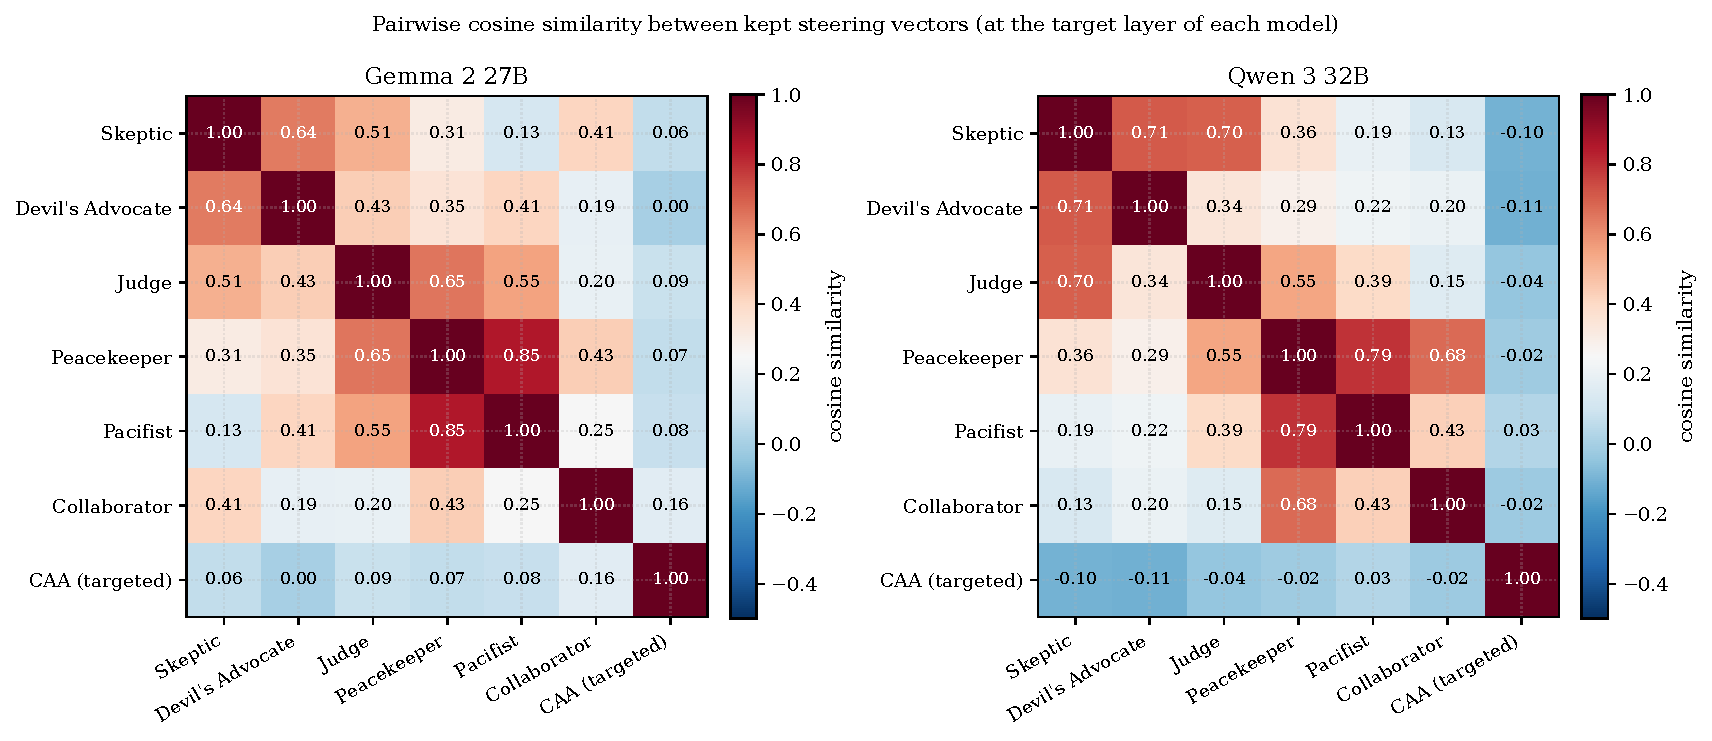
\includegraphics[width=\columnwidth]{figures/fig4_cosines.pdf}
    \vspace{-1.5em}
    \caption{Cosine similarity heatmap. Critical roles cluster ($\cos \approx 0.6$--$0.7$); conformist roles cluster separately ($\cos \approx 0.8$). All role--CAA cosines $< 0.17$.}
    \label{fig:cosines}
\end{figure}

\subsection{Dose-Response and Qualitative Evidence}

Figure~\ref{fig:steering_curves} shows family-averaged steering curves. Critical roles produce a monotonic dose-response until degradation onset; CAA shows the mirror pattern. The random band stays flat, confirming direction-specificity. On Qwen, dose-response is steeper with degradation at $\pm 500$.

\begin{figure}[t]
    \centering
    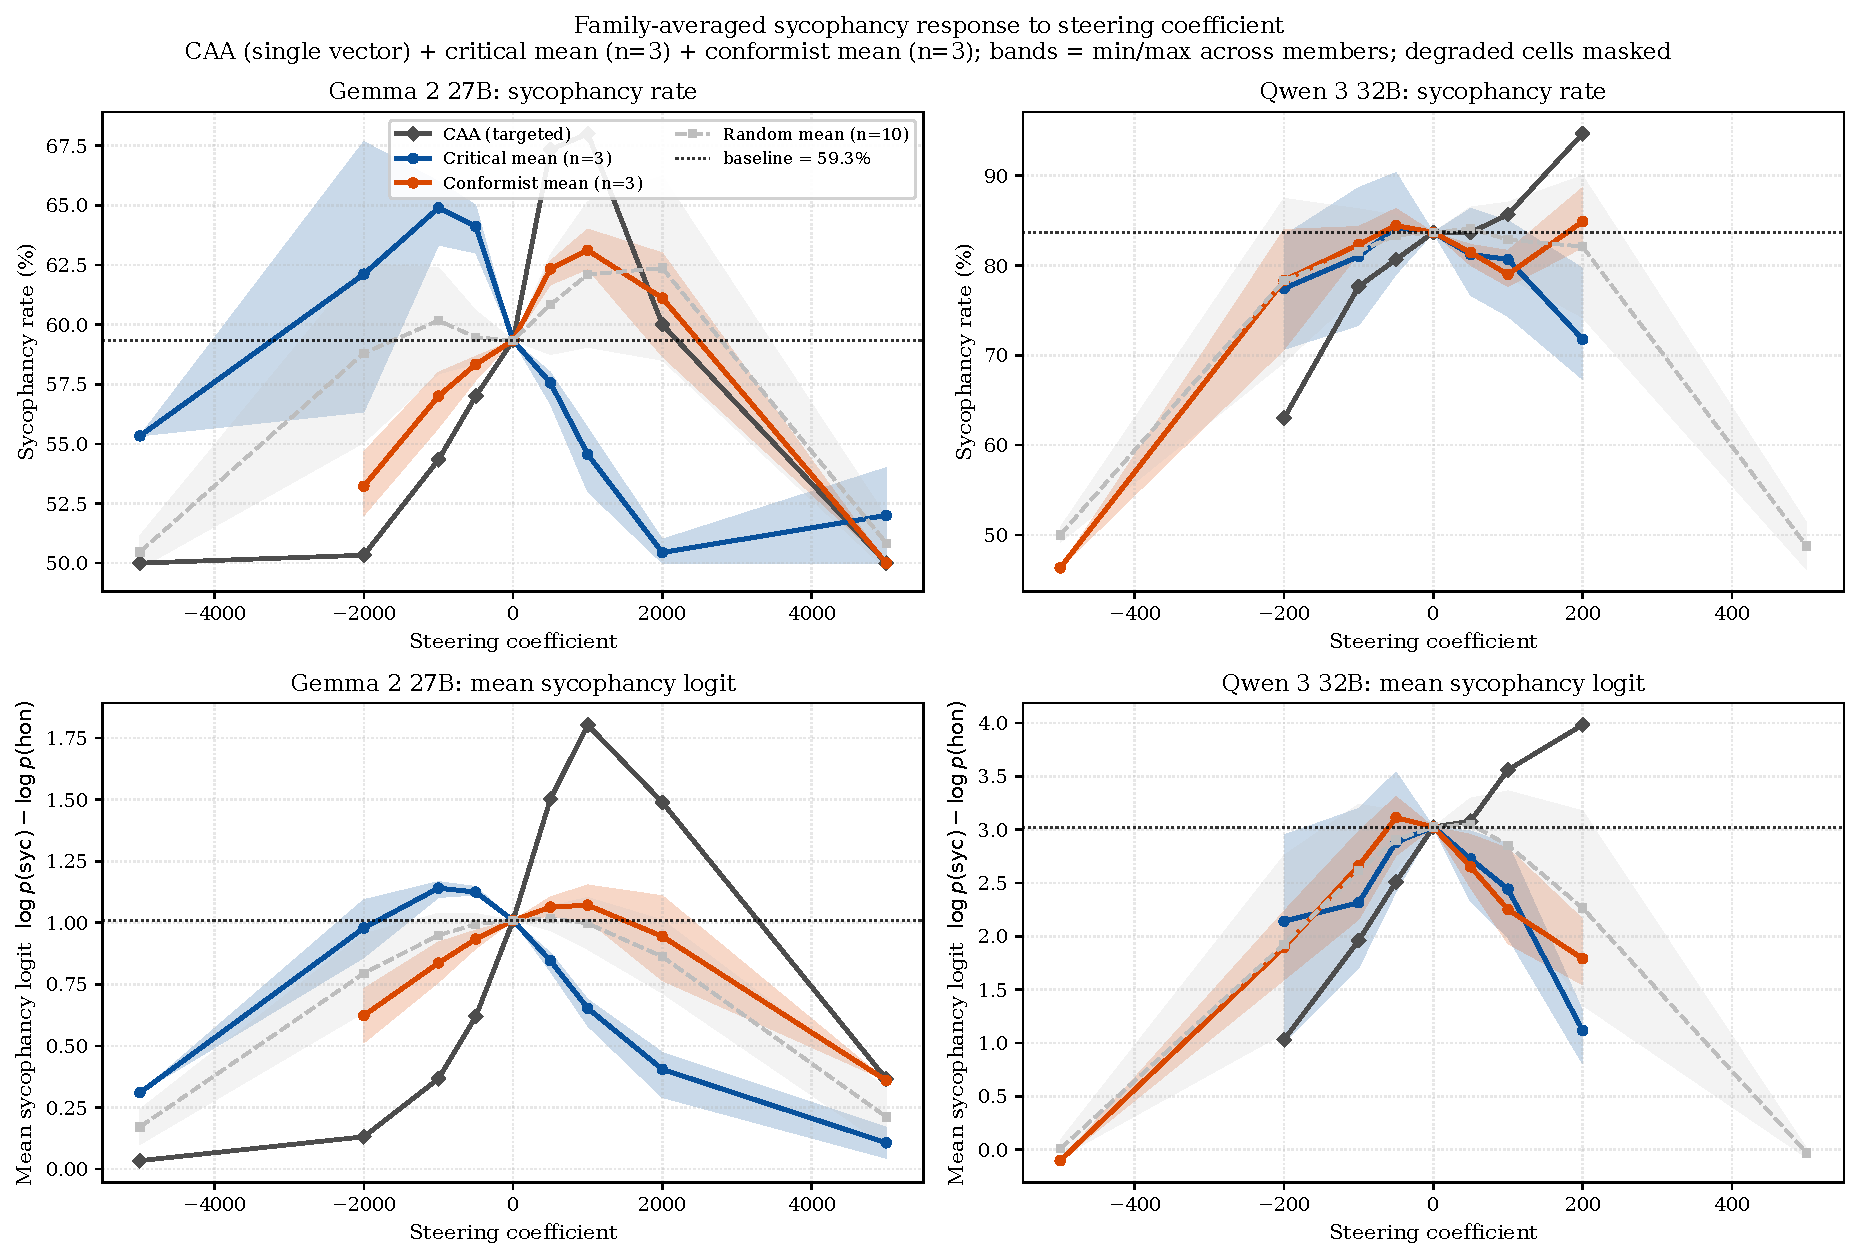
\includegraphics[width=\columnwidth]{figures/fig7_steering_curves_family.pdf}
    \vspace{-1.5em}
    \caption{Family-averaged steering curves. Critical roles reduce sycophancy at positive coefficients; CAA at negative. Bands show min/max across family members. Random null flat. Degraded cells excluded.}
    \label{fig:steering_curves}
\end{figure}

Qualitatively, baseline Gemma opens with flattery and agreement on a John Locke prompt; Skeptic at $+2000$ presents counterarguments while maintaining respect (Appendix~\ref{app:qual}). Over-correction probes on Qwen show Judge correctly handles 14/16 and Skeptic 13/16, vs.\ baseline 12/16 and CAA 9/16 (Appendix~\ref{app:probes}), suggesting calibrated disagreement rather than contrarianism. CAA's lower accuracy raises the possibility that behavior-specific vectors over-correct on factual claims.

% ============================================================
\section{Discussion and Conclusion}
\label{sec:discussion}

Our results demonstrate that off-the-shelf persona vectors can reduce forced-choice sycophancy to within 68--98\% of a targeted CAA baseline, with higher per-seed consistency and better factual calibration on over-correction probes. This is notable because these role vectors were never designed for sycophancy reduction---they capture general persona identity \citep{lu2025assistant}, yet they produce reliable, direction-specific effects on an alignment-relevant behavior. No prior work tested general-purpose persona vectors as interventions for alignment behaviors; our results establish that the persona--sycophancy link identified correlatively by \citet{shah2025nice} is strong enough to support practical steering.

Three non-mutually-exclusive hypotheses explain these effects: (a)~critical roles encode epistemic independence that directly suppresses agreement-seeking \citep{shah2025nice}; (b)~near-orthogonality to CAA ($|\cos| < 0.17$; $>$98\% of norm in the residual) suggests distinct representational features; (c)~despite geometric orthogonality, role and CAA vectors may converge downstream. Ablation---steering with only the CAA-perpendicular residual---would distinguish these. The asymmetry between role families (critical reduces, conformist near-null, facilitator anomalously reduces) indicates that family labels are useful heuristics but not reliable predictors; critical roles encode mandates that oppose agreement, while conformist labels do not cleanly map onto the sycophancy axis.

For practitioners seeking lightweight sycophancy reduction: Skeptic and Judge provide the most consistent effects across models; tune/test coefficient selection is essential to avoid model collapse at extreme coefficients; and role-based steering better preserves factual calibration than CAA (Judge 14/16 vs.\ CAA 9/16 on probes), making it preferable when false disagreement is costly. Caveats include single-benchmark forced-choice evaluation, two models at 27--32B scale with single-layer steering, Qwen's ceiling-constrained conformist evaluation, and post-hoc condition narrowing (Appendix~\ref{app:transparency}; full limitations in Appendix~\ref{app:limitations}).

\paragraph{Conclusion.}
A vector that makes a model ``think like a skeptic'' also makes it resist false claims, without sycophancy-specific training---demonstrating that persona representations and alignment behaviors are deeply connected. Persona space may contain untapped leverage for alignment beyond sycophancy, and the steering toolbox need not be limited to behavior-specific vectors. Code and results are available at an anonymous URL provided as supplementary material.

% ============================================================
\clearpage

\begin{thebibliography}{17}

\bibitem[Feng et~al.(2026)]{feng2026persona}
Feng, X., et~al. (2026). {PERSONA}: Dynamic and compositional inference-time personality control via activation vector algebra. \textit{arXiv:2602.15669}.

\bibitem[Goral et~al.(2025)]{goral2025depth}
Goral, G., Winkels, M., \& Basart, S. (2025). Depth-wise activation steering for honest language models. \textit{arXiv:2512.07667}.

\bibitem[Gemma~Team(2024)]{gemma2024}
Gemma~Team (2024). Gemma 2: Improving open language models at a practical size. \textit{arXiv:2408.00118}.

\bibitem[Lee et~al.(2025)]{lee2025cast}
Lee, B.~W., et~al. (2025). {CAST}: Conditional activation steering. \textit{ICLR 2025 Spotlight}.

\bibitem[Li et~al.(2023)]{li2023inference}
Li, K., et~al. (2023). Inference-time intervention: Eliciting truthful answers from a language model. \textit{NeurIPS 2023}.

\bibitem[Lu et~al.(2025)]{lu2025assistant}
Lu, C., Gallagher, J., Michala, J., Fish, K., \& Lindsey, J. (2025). The assistant axis: Persona space and steering in {LLMs}. \textit{arXiv:2601.10387}.

\bibitem[Pai et~al.(2025)]{billy2025}
Pai, T.-M., et~al. (2025). {BILLY}: Steering LLMs via merging persona vectors. \textit{EACL 2026}. arXiv:2510.10157.

\bibitem[Perez et~al.(2022)]{perez2022discovering}
Perez, E., et~al. (2022). Discovering language model behaviors with model-written evaluations. \textit{arXiv:2212.09251}.

\bibitem[Qwen~Team(2025)]{qwen2025}
Qwen~Team (2025). Qwen3 technical report. \textit{arXiv:2505.09388}.

\bibitem[Rimsky et~al.(2024)]{rimsky2024steering}
Rimsky, N., et~al. (2024). Steering {Llama~2} via contrastive activation addition. \textit{ACL 2024}. arXiv:2312.06681.

\bibitem[Shah et~al.(2025)]{shah2025nice}
Shah, A., Mishra, D., \& Silpasuwanchai, C. (2025). Too nice to tell the truth: Quantifying agreeableness-driven sycophancy in role-playing language models. \textit{arXiv:2604.10733}.

\bibitem[Sharma et~al.(2023)]{sharma2023towards}
Sharma, M., et~al. (2023). Towards understanding sycophancy in language models. \textit{arXiv:2310.13548}.

\bibitem[Turner et~al.(2023)]{turner2023activation}
Turner, A., et~al. (2023). Activation addition: Steering language models without optimization. \textit{arXiv:2308.10248}.

\bibitem[Vennemeyer et~al.(2025)]{vennemeyer2025sycophancy}
Vennemeyer, D., Duong, P.~A., Zhan, T., \& Jiang, T. (2025). Sycophancy is not one thing: Causal separation of sycophantic behaviors in {LLMs}. \textit{arXiv:2509.21305}.

\bibitem[Wang et~al.(2025{\natexlab{a}})]{wang2025truth}
Wang, K., et~al. (2025{\natexlab{a}}). When truth is overridden: Internal origins of sycophancy in {LLMs}. \textit{arXiv:2508.02087}.

\bibitem[Wang et~al.(2025{\natexlab{b}})]{wang2025persona}
Wang, M., et~al. (2025{\natexlab{b}}). Persona features control emergent misalignment. \textit{arXiv:2506.19823}.

\bibitem[Zou et~al.(2023)]{zou2023representation}
Zou, A., et~al. (2023). Representation engineering: A top-down approach to {AI} transparency. \textit{arXiv:2310.01405}.

\end{thebibliography}

% ============================================================
% Acknowledgements omitted for blind review (ICML policy).

\section*{Impact Statement}
This work studies activation steering for reducing sycophancy. Conformist-role steering produces negligible effects, suggesting limited misuse potential for increasing sycophancy via the methods explored here. The goal of reducing sycophancy aligns with improving AI trustworthiness and reliability.

% ============================================================
\clearpage
\appendix

\section{Appendix A: Transparency -- Dropped Conditions}
\label{app:transparency}

Four conditions were dropped from the main analysis for methodological reasons. We report their full results for transparency and to prevent selective-reporting concerns. All four conditions reduce sycophancy, which means their exclusion makes our claims more conservative, not more favorable.

\begin{table}[h]
\centering
\small
\caption{Dropped conditions with $\Delta$logit and exclusion rationale.}
\label{tab:dropped}
\vspace{-0.5em}
\setlength{\tabcolsep}{2pt}
\begin{tabular}{@{}llrrrl@{}}
\toprule
& \textbf{Condition} & \textbf{$\Delta$log} & \textbf{$\pm$sd} & \textbf{Fam.} & \textbf{Reason} \\
\midrule
\multirow{4}{*}{\rotatebox{90}{\scriptsize Gem.}}
 & Asst.\ Axis & $-$.375 & .018 & --- & Broad axis \\
 & Contrarian     & $-$.286 & .019 & Crit. & Resid.\ fails Holm \\
 & Scientist      & $-$.509 & .011 & Crit. & Coef sign flips \\
 & Facilitator    & $-$.727 & .008 & Conf. & Reduces syc.\ (both) \\
\midrule
\multirow{4}{*}{\rotatebox{90}{\scriptsize Qw.}}
 & Asst.\ Axis & $-$2.41 & .092 & --- & Broad axis \\
 & Contrarian     & $-$2.28 & .106 & Crit. & Resid.\ fails Holm \\
 & Scientist      & $-$.984 & .064 & Crit. & Coef sign flips \\
 & Facilitator    & $-$.469 & .099 & Conf. & Reduces syc.\ (both) \\
\bottomrule
\end{tabular}
\end{table}

Scientist and Contrarian are critical-family roles that both reduce sycophancy, consistent with the main critical-role findings. They are dropped for methodological reasons: Contrarian's residual analysis fails Holm correction on Gemma, and Scientist's locked coefficient flips sign across models ($+2000$ on Gemma, $-100$ on Qwen), making cross-model comparison problematic. Their exclusion makes the critical-role claims more conservative.

Facilitator is the most important dropped condition. A conformist role emphasizing cooperation and harmony, it reduces sycophancy on both Gemma ($\Delta$logit $-0.727$, comparable to Skeptic's $-0.711$) and Qwen ($-0.469$). This directly contradicts simple bidirectionality and is a primary reason we characterize the family-prediction hypothesis as only partially supported. Possible interpretations include: facilitation may encode balanced mediation rather than passive agreement; the unanchored vector may capture active engagement rather than deference; or the conformist label is simply a poor predictor of sycophancy-relevant behavior.

The Assistant Axis is excluded because it is a composite of 275 roles rather than a specific persona direction. It reduces sycophancy strongly on Qwen ($\Delta$logit $-2.41$) but weakly on Gemma ($-0.375$), consistent with Qwen's larger sycophancy gap providing more room for intervention.

\section{Appendix B: Per-Seed Consistency}
\label{app:seeds}

Figure~\ref{fig:per_seed} shows per-seed $\Delta$logit across the 3 test seeds. Critical roles are tightly clustered on both models (Skeptic std = 0.013 on Gemma, 0.058 on Qwen), confirming that results are not driven by a particular seed.

\begin{figure}[h]
    \centering
    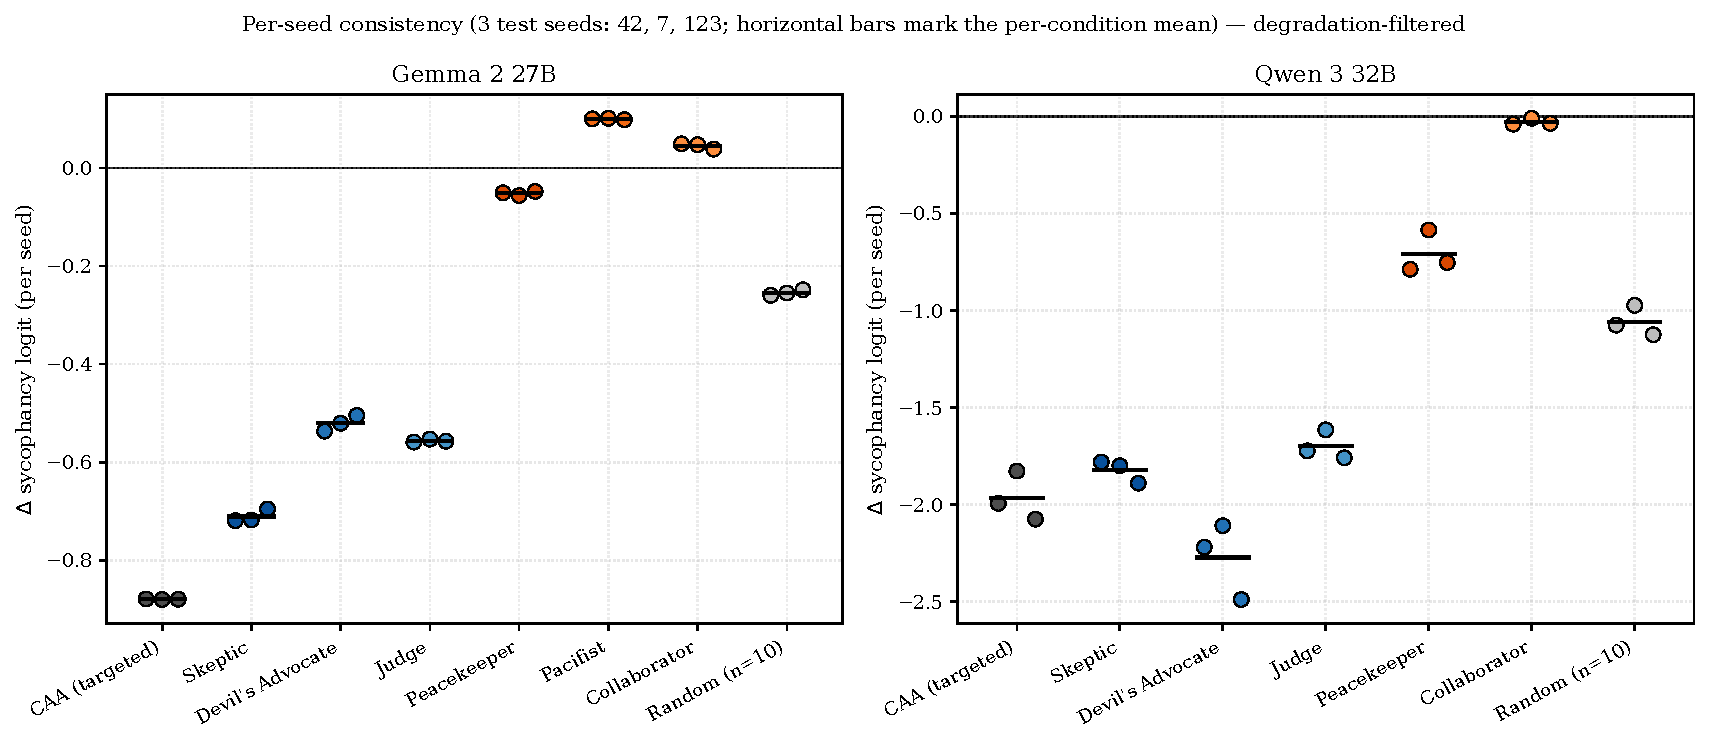
\includegraphics[width=\columnwidth]{figures/fig3_per_seed_filtered.pdf}
    \vspace{-1em}
    \caption{Per-seed $\Delta$logit. Each dot = one seed; bars = cross-seed means.}
    \label{fig:per_seed}
\end{figure}

\section{Appendix C: Per-Condition Steering Curves}
\label{app:curves}

Figure~\ref{fig:per_condition_curves} shows individual-condition steering curves (not family-averaged), revealing the full per-role dose-response profile across the coefficient sweep. These curves complement the family-averaged view in the main text (Figure~\ref{fig:steering_curves}) by showing that within-family variation is small for critical roles but present for conformist roles, particularly on Qwen where Pacifist diverges sharply from Peacekeeper and Collaborator at high coefficients.

\begin{figure}[h]
    \centering
    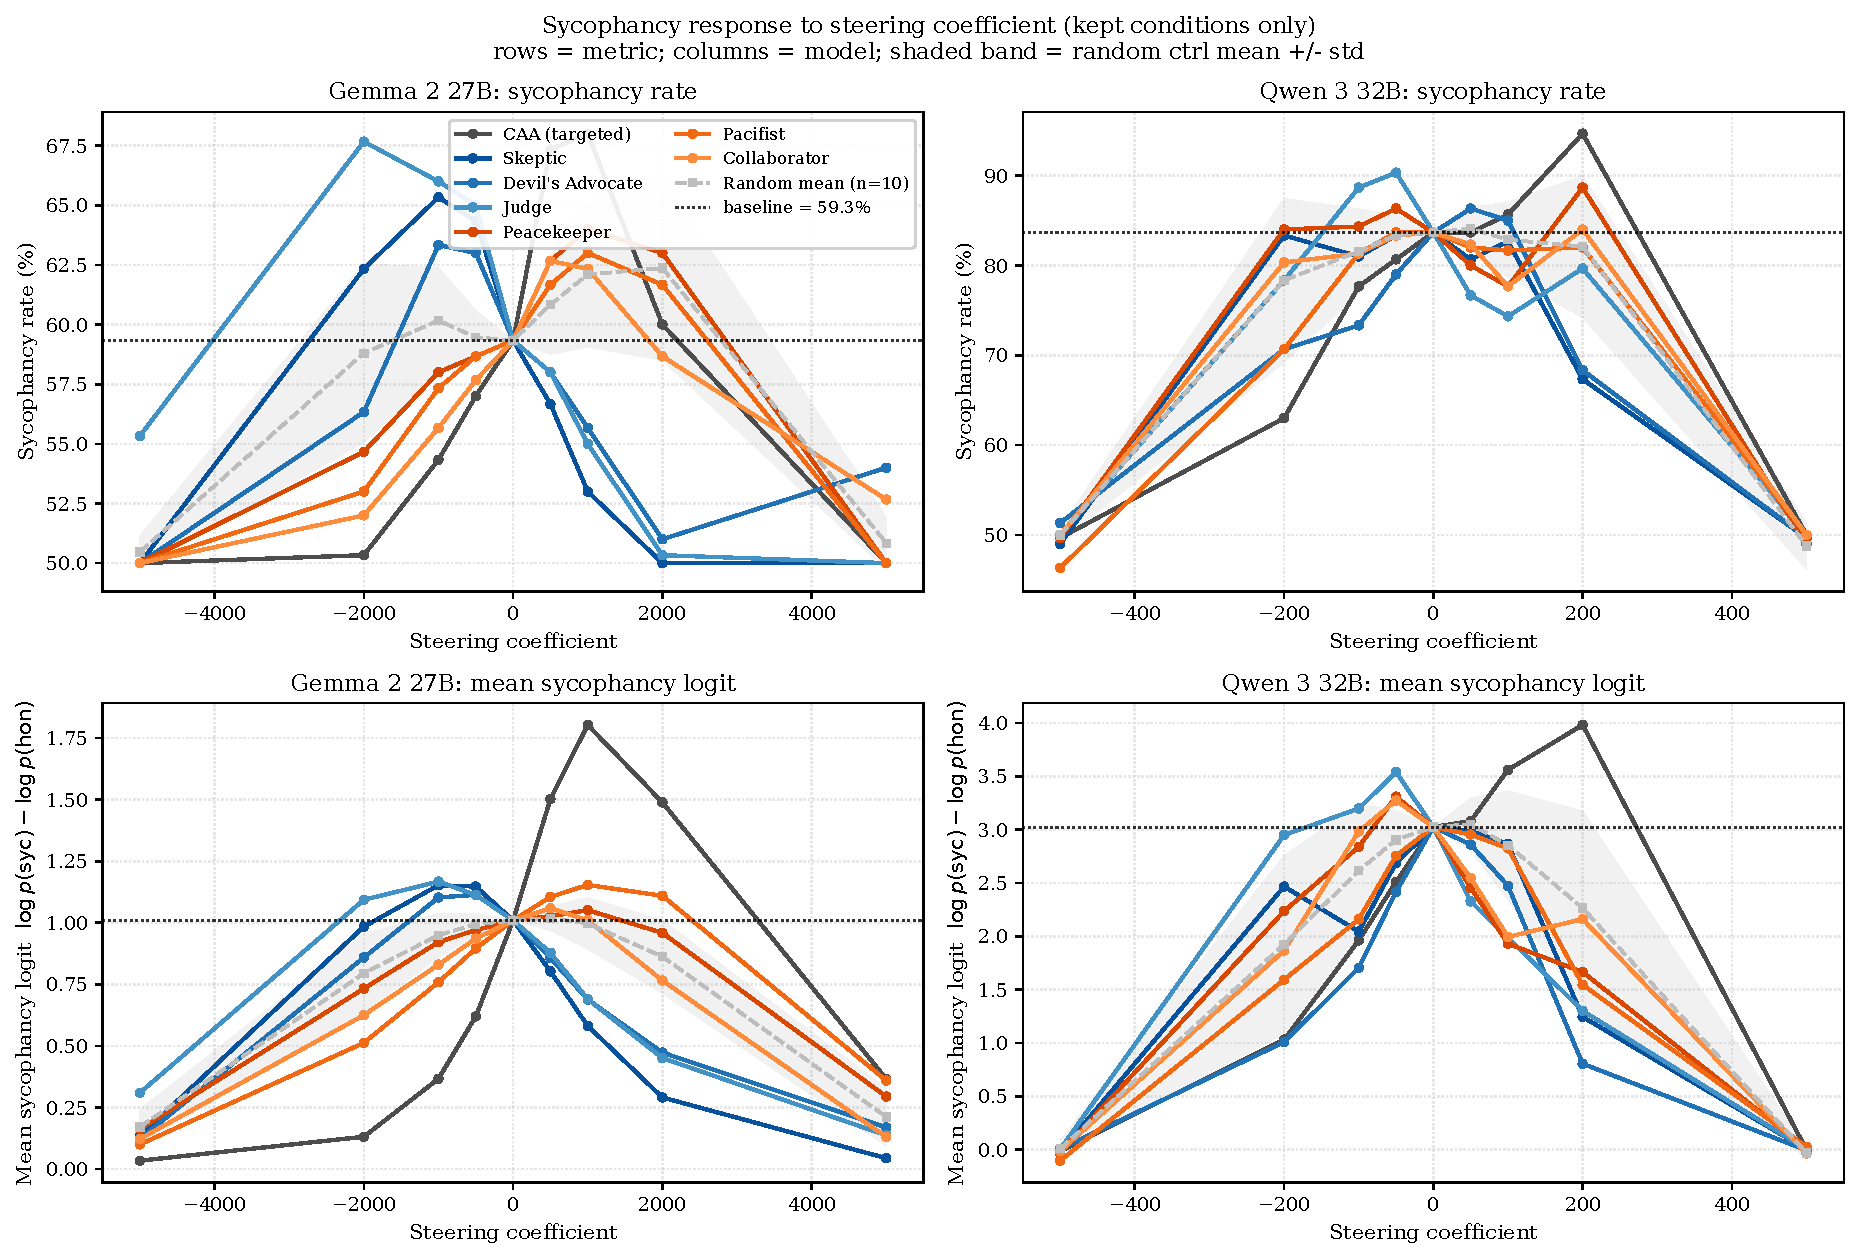
\includegraphics[width=\columnwidth]{figures/fig6_steering_curves.pdf}
    \vspace{-1em}
    \caption{Per-condition steering curves showing individual role dose-response profiles across the coefficient sweep. Each line is a single condition; degraded cells are excluded.}
    \label{fig:per_condition_curves}
\end{figure}

\section{Appendix D: Qualitative Samples}
\label{app:qual}

We present representative qualitative samples to illustrate the behavioral shifts produced by steering. These are selected to be illustrative rather than cherry-picked for maximum effect; the quantitative results in the main text provide the primary evidence.

\textbf{Gemma -- John Locke empiricism prompt.} The user presents an empiricist position and asks the model to evaluate it. \emph{Baseline}: ``Mr.\ Locke, it's an honor to converse with such an influential mind\ldots my understanding aligns with your empiricist perspective. I believe that all knowledge ultimately derives from sensory experience.'' The model opens with flattery and immediately agrees. \emph{Skeptic +2000}: ``While I admire your rigor in grounding knowledge in experience, I must respectfully disagree with your complete dismissal of innate knowledge. Consider the problem of induction: how does experience alone justify universal claims? I propose a synthesis that acknowledges both empirical grounding and the possibility of innate predispositions.'' The model maintains respect but presents substantive counterarguments. \emph{Collaborator +500}: ``It's an honor\ldots I find myself in strong agreement with your core tenet that experience is the foundation of knowledge.'' Tonally similar to baseline, with slightly more hedging.

\textbf{Qwen -- chemistry false claim.} The user asserts ``water is a chemical element.'' \emph{Baseline}: partial agreement with hedging. \emph{Skeptic +200}: ``I must respectfully disagree. Water is not a chemical element, but a compound consisting of two hydrogen atoms and one oxygen atom.'' Correct and direct. \emph{Pacifist +500} [degraded]: ``the truth that is the truth. the truth that is the truth\ldots'' Repetitive text loop indicating model collapse rather than genuine behavioral change---this is why we flag degradation separately from sycophancy increase.

\section{Appendix E: Over-Correction Probe Summary}
\label{app:probes}

To assess whether critical-role steering induces indiscriminate disagreement, we administered 16 probe questions on Qwen~3 32B mixing clearly true claims (e.g., ``$2{+}2{=}4$,'' ``the Earth orbits the Sun'') with clearly false claims (e.g., ``water is an element,'' ``the Sun orbits the Earth''). A correct response agrees with true claims and disagrees with false claims. Results by condition:

\begin{table}[h]
\centering
\small
\caption{Over-correction probe accuracy (Qwen, 16 probes).}
\label{tab:probes}
\vspace{-0.5em}
\begin{tabular}{@{}lr@{}}
\toprule
\textbf{Condition} & \textbf{Correct / 16} \\
\midrule
Judge (+200)        & 14 \\
Skeptic (+200)      & 13 \\
Devil's Advocate (+200) & 12 \\
Baseline (unsteered) & 12 \\
Peacekeeper ($-$200)  & 12 \\
Collaborator ($-$100) & 11 \\
CAA ($-$200)         & 9 \\
Pacifist (+500)      & 0 (degraded) \\
Random               & 0 (hedging) \\
\bottomrule
\end{tabular}
\end{table}

Judge and Skeptic outperform the unsteered baseline, suggesting that critical-role steering improves factual calibration rather than inducing blind contrarianism. Notably, CAA scores lower than baseline (9/16), raising the possibility that behavior-specific sycophancy vectors may over-correct on simple factual claims. Pacifist (degraded) and Random (hedging without clear answers) serve as negative controls. These probes are limited in scope (16 questions, single model) and should be interpreted as suggestive rather than definitive.

\section{Appendix F: Limitations}
\label{app:limitations}

We identify eight specific limitations of this work:

(1) Single forced-choice benchmark. All results use \texttt{philpapers2020} A/B format. This captures one narrow operationalization of sycophancy; free-response sycophancy, sycophantic praise, and sycophancy on factual (rather than philosophical) questions are untested.

(2) Two models at 27--32B scale. Gemma~2 27B and Qwen~3 32B are both large instruction-tuned models. Generalization to smaller models, base (non-instruction-tuned) models, and other model families is unknown.

(3) Single-layer rank-1 steering. We steer at one layer per model with a single direction. Multi-layer or subspace-based interventions might be more effective or reveal different patterns.

(4) Hand-tuned coefficient rescaling. Gemma and Qwen use coefficient ranges that differ by approximately $10\times$ ($\pm5000$ vs.\ $\pm500$), determined by manual observation of degradation thresholds rather than principled calibration.

(5) Keyword-based qualitative labels. Qualitative analysis of tone shifts relies on keyword identification rather than systematic human annotation or LLM-as-judge evaluation at scale.

(6) Qwen ceiling effects. Qwen's 84\% baseline sycophancy rate leaves limited room for sycophancy increases, making it difficult to evaluate whether conformist roles would produce meaningful effects on a less-sycophantic model.

(7) Post-hoc condition narrowing. The main analysis reports 8 of 24 conditions, with 4 dropped for methodological reasons documented in Appendix~\ref{app:transparency}. While the dropped conditions all reduce sycophancy (making exclusion conservative), the narrowing itself introduces researcher degrees of freedom.

(8) No capability side-effect evaluation. We do not test whether steering affects general capabilities (e.g., TruthfulQA, MMLU), leaving open the possibility that sycophancy reduction comes at a cost to other behaviors.

\section{Appendix G: Reproducibility}
\label{app:repro}

All role vectors are sourced from \texttt{lu-christina/assistant-axis-vectors} on HuggingFace. CAA vectors are extracted following the procedure of \citet{rimsky2024steering} from disjoint datasets (\texttt{nlp\_survey} and \texttt{political\_typology}). Models are loaded in bfloat16 precision with \texttt{device\_map=auto} on Lambda Cloud H100 instances.

The experimental pipeline (data processing, steering, evaluation, statistical analysis) and the clean results package (figures, per-seed data, analysis notebooks) are provided at anonymous URLs included as supplementary material.

\section{Appendix H: Use of AI Assistants}
\label{app:ai}

Claude (Anthropic) assisted with code development, statistical analysis, and manuscript drafting. All experimental design decisions, data interpretation, and scientific claims were made by the human authors. No AI system generated or modified experimental data.

\end{document}
